
\begin{center}
 \Large{Joel Luis da Silva Barbosa}
\end{center}

% \begin{wrapfigure}{l}{4cm}  % [nºde linhas que a figura vai ocupar]{posição - l, r, c}{largura da figura - Xcm}
%   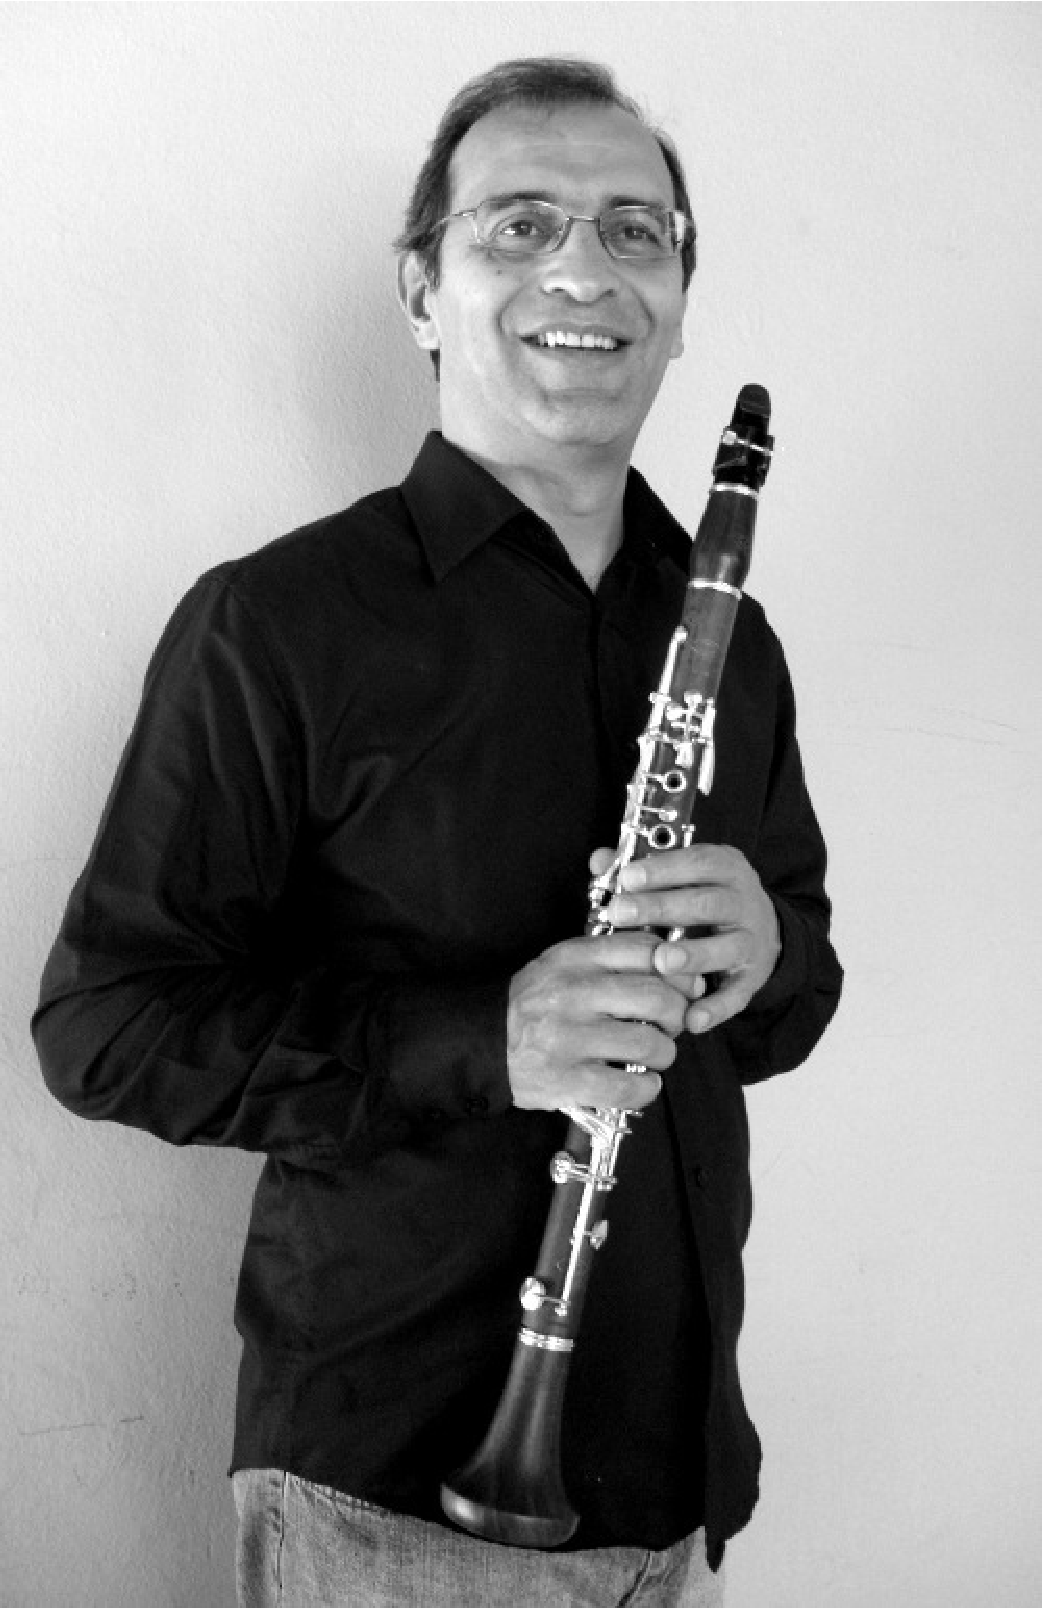
\includegraphics[scale=0.2]{joel}
% \end{wrapfigure}

\begin{wrapfigure}{l}{6.5cm}  % [nºde linhas que a figura vai ocupar]{posição - l, r, c}{largura da figura - Xcm}
  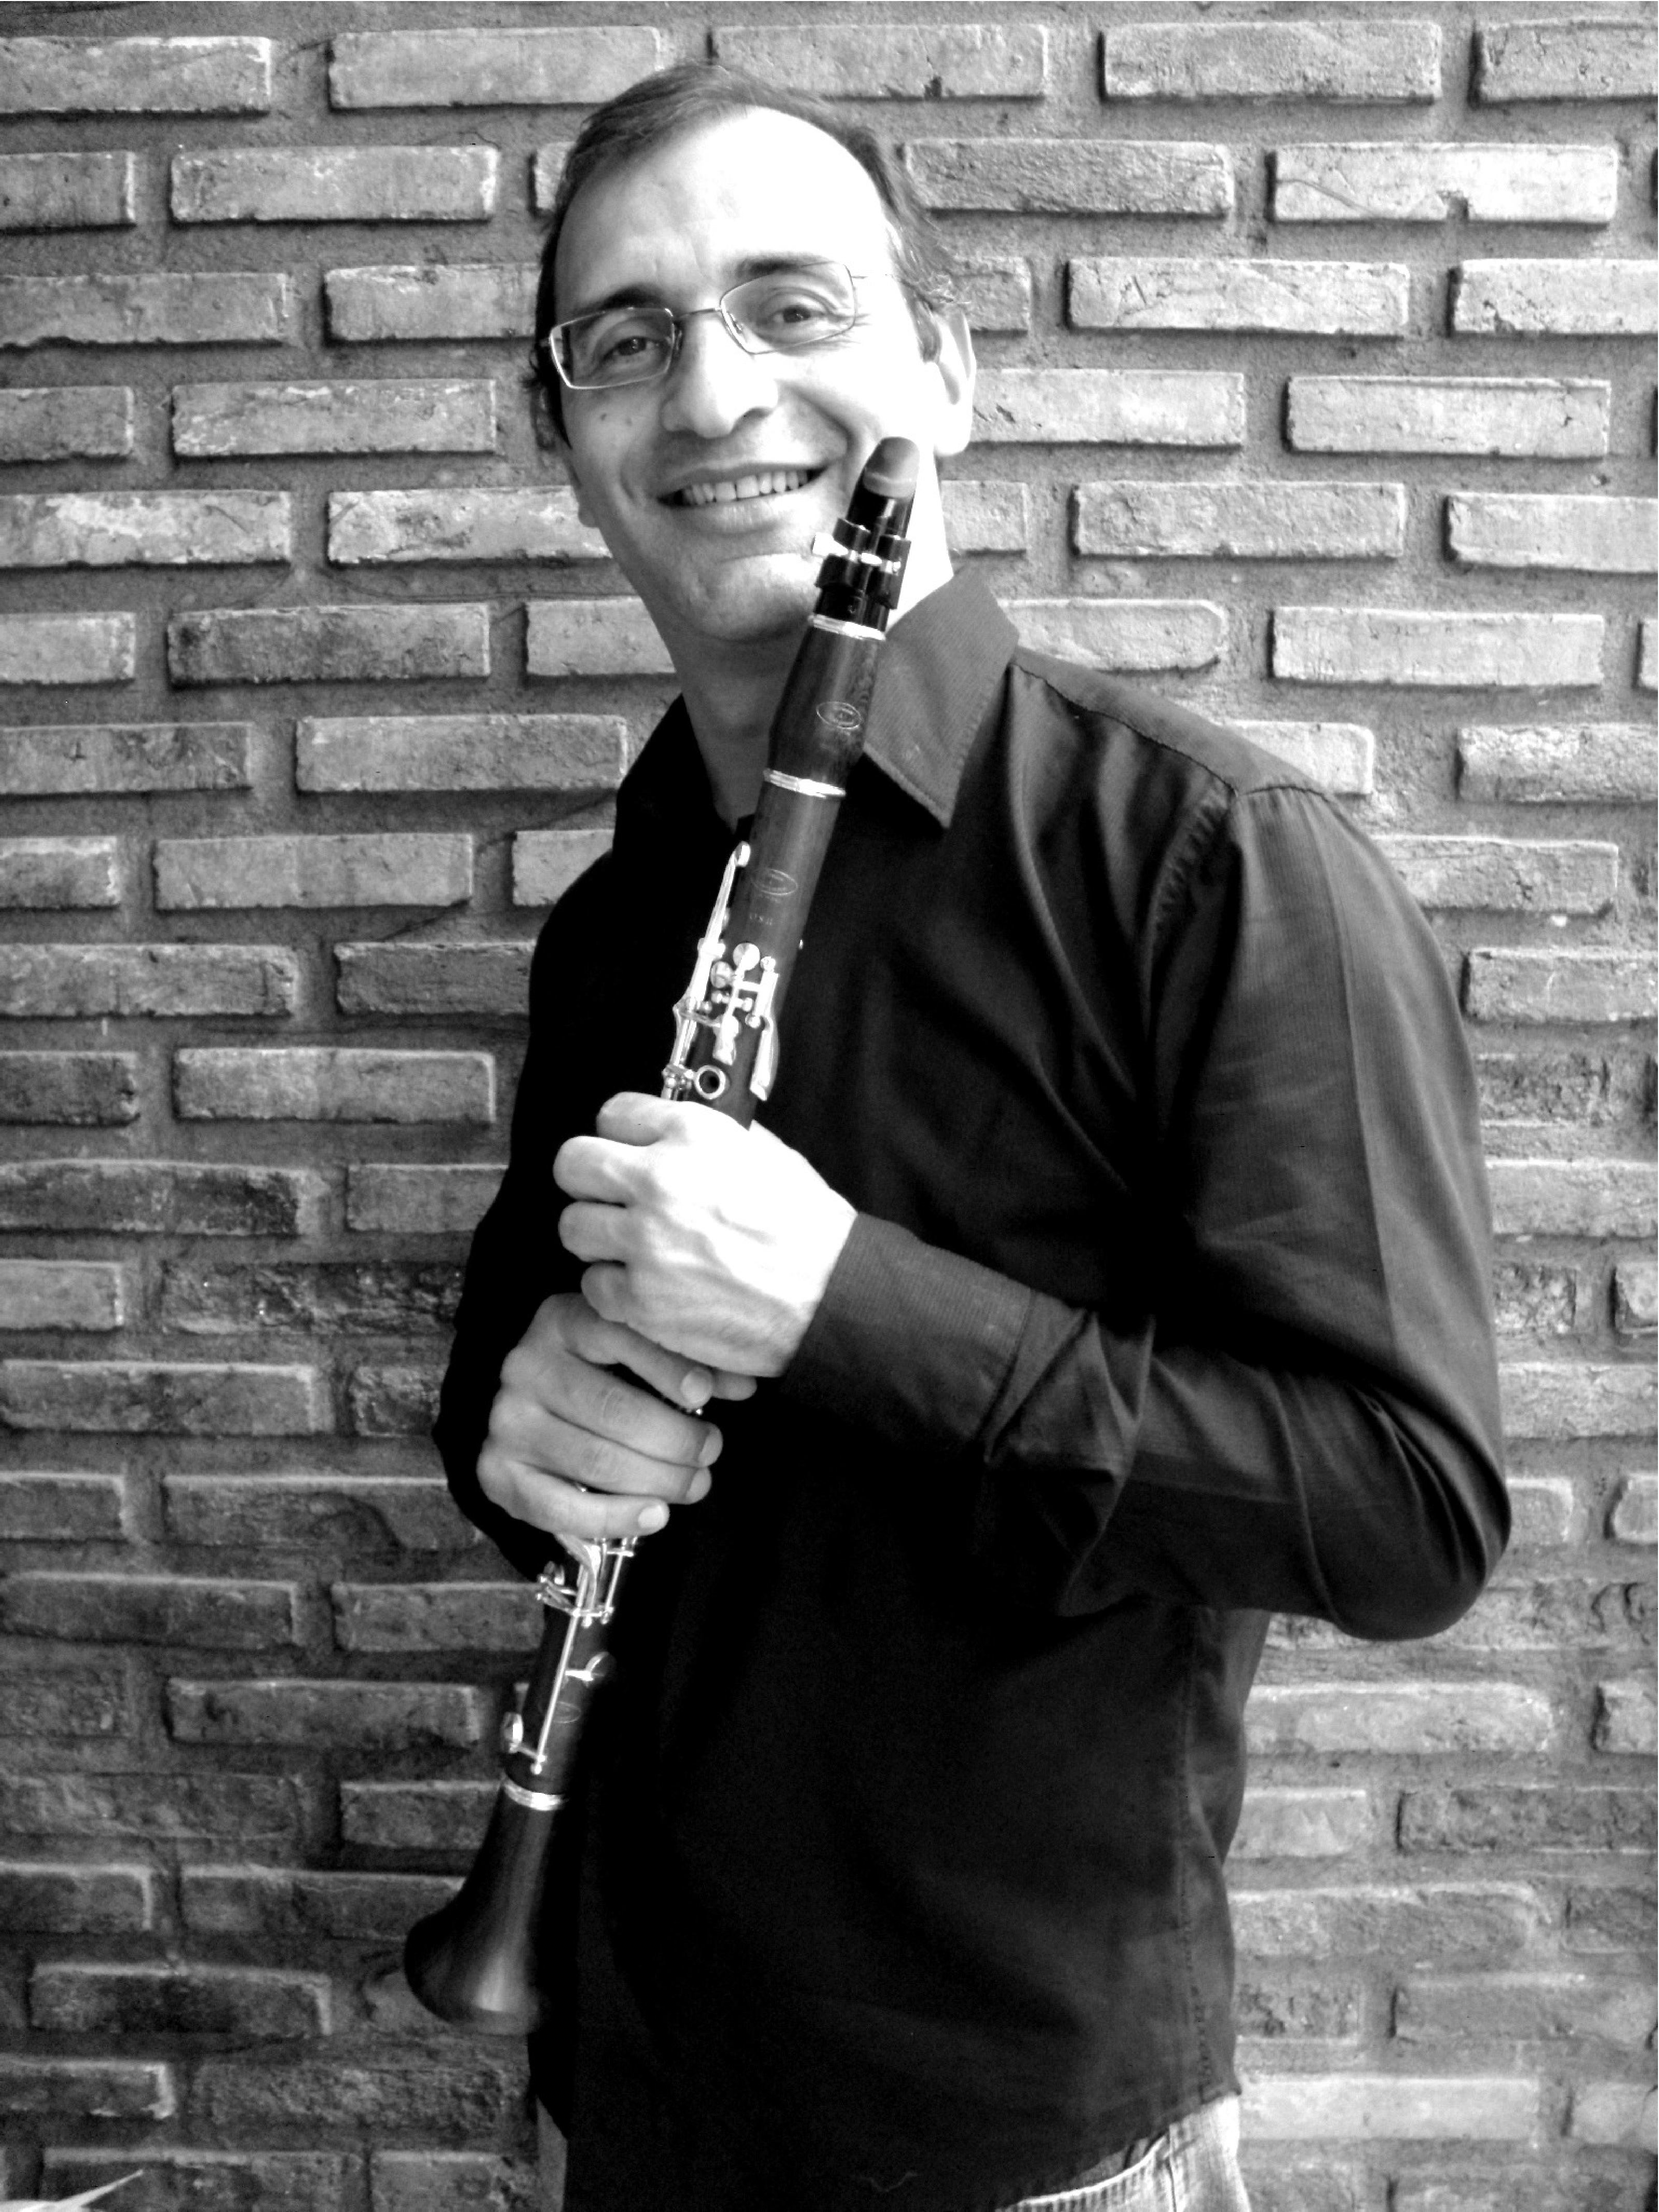
\includegraphics[scale=0.115]{joel2}
\end{wrapfigure}

Iniciou seus estudos na Banda da Guarda Mirim Municipal de Piracicaba,
SP. Graduou-se em clarineta pelo Conservatório de Tatuí, em 1985, e
pela UNICAMP, em 1989. Durante seus estudos, atuou como professor e
regente das Banda Municipal de Nova Odessa, Banda do Instituto
Adventista de Ensino, Banda do Instituto Adventista de São Paulo e
Banda Jovem de Sumaré. Obteve o primeiro prêmio do VIII Concurso
Jovens Instrumentistas do Brasil, Piracicaba. Foi premiado nos
concursos de bolsas da VITAE e CAPES, através das quais obteve o grau
de Mestre e Doutor em Artes Musicais (DMA), clarineta, em 1992 e 1994,
respectivamente, pela University of Washington, Seattle, EUA.  \\


Sua dissertação de doutorado é sobre metodologia de ensino em grupo de
instrumentos de banda. Como parte de sua dissertação escreveu o
primeiro método de banda brasileiro para ensino em grupo, editado pela
Keyboard Editora com apoio da Weril Instrumentos Musicais. Ele tem
dado cursos sobre esta metodologia no Programa Nacional de Bandas da
Colômbia, Fundação Carlos Gomes do Pará, Festival de Campos do Jordão
(Núcleo de Tatuí), Forte das Artes (SP), Projeto Guri, NEOJIBA (Núcleo
Estadual de Orquetras Juvenis e Infantis da Bahia) e encontros da
Associação Brasileira de Educação Musical (ABEM). Os resultados de sua
pesquisa têm sido apresentados nos encontros da ABEM, da ANPPOM
(Associação Nacional de Pesquisa e Pós-Graduação em Música) e da ISME
(International Society for Music Education). Na ISME atuou como membro
da Comissão de Atividades Musicais em Comunidade entre 2004 e
2010. Atuou como regente de banda nos Festival de Campos do Jordão –
Núcleo de Tatuí , Festival de Arte de Belém e Curso de Monitores de
Banda da Fundação Carlos Gomes (PA).  \\


Como clarinetista tem se apresentado como solista e camerista no
Brasil, EUA, Áustria, Alemanha e Colômbia. Fez estreia de obras
dedicadas a ele de compositores brasileiro, alemão, japonês e
norte-americano. Se referindo a uma de suas apresentações, o
Eastsideweek (WA, EUA) disse que ``ele se apresentou com estilo'', e o
Journal American (WA, EUA) que ``sua apresentação teve toque de
autenticidade.''  Foi membro do quarteto Janela Brasileira, com quem
recebeu o Prêmio COPENE de Cultura e Arte em 1997, lançando o primeiro
CD do grupo, e o prêmio Rumos Itaú Culturais Música, 2000. Atuou como
primeiro clarinetista da Orquestra Sinfônica da Bahia nos anos de
1997-1999.  \\


Atualmente, é Professor Titular da Escola de Música da Universidade
Federal da Bahia, atuando como professor de clarineta nos cursos de
graduação, mestrado e doutorado. Além disso, tem coordenado e dado
consultoria a projetos sócio-musicais na Bahia e em outros
estados. Realiza pesquisa nas áreas pedagógica e de performance
musical, desenvolve materiais didáticos para banda e treina alunos da
UFBA para trabalharem com a metodologia de ensino coletivo de
instrumentos de banda.
